% !TEX root = ../main.tex
\chapter{Therminator model}
  \verb|THERMINATOR|~\cite{therminator} is a Monte Carlo event generator designed to investigate the particle production in the relativistic heavy ion collisions.
  The functionality of the code includes a generation of the stable particles and unstable resonances at the chosen hypersurface model.
  It performs the statistical hadronization which is followed by space-time evolution of particles and the decay of resonances.
  The key element of this method is an inclusion of a complete list of hadronic resonances, which contribute very significantly to the observables.
  The second version of \verb|THERMINATOR|~\cite{therminator2} comes with a posibility to incorporate any shape of freeze-out hypersurface and the expansion velocity field, especially those generated externally with various hydrodynamic codes.

  %
  % ========
  \section{(3+1)-dimensional viscous hydrodynamics}
  % ========
  Most of the relativistic viscous hydrodynamic calculations are done in \mbox{(2+1)-dimensions}.
  Such simplification assumes boost-invariance of a matter created in a collision.
  Experimental data reveals that no boost-invariant region is formed in the collisions~\cite{chmeson}.
  Hence, for the better description of created system a \mbox{(3+1)-dimensional} model is required.

  In the four dimensional relativistic dynamics one can describe a system using a space-time four-vector $x^\nu=(ct,x,y,z)$, a velocity four-vector $u^\nu=\gamma(c,v_x,v_y,v_z)$ and a energy-momentum tensor $T^{\mu\nu}$.
  The particular components of $T^{\mu\nu}$ have a following meaning:
  \begin{itemize}
    \item $T^{00}$ - an energy density,
    \item $c T^{0\alpha}$ - an energy flux across a surface $x^\alpha$,
    \item $T^{\alpha0}$ - an $\alpha$-momentum flux across a surface  $x^\alpha$ multiplied by $c$,
    \item $T^{\alpha\beta}$ - components of momentum flux density tensor,
  \end{itemize}
  where $\gamma = (1-v^2/c^2)^{-1/2}$ is Lorentz factor and $\alpha,\beta \in \{1,2,3\}$.
  Using $u^\nu$ one can express $T^{\mu\nu}$ as follows~\cite{israel}:
  \begin{equation}
    \label{eq:visc_ten}
    T^{\mu\nu}_0 = (e+p)u^\mu u^\nu - pg^{\mu\nu}
  \end{equation}
  where $e$ is an energy density, $p$ is a pressure and $g^{\mu\nu}$ is an inverse metric tensor:
  \begin{equation}
    g^{\mu\nu} = 
    \begin{bmatrix}
      1 & 0 & 0 & 0 \\
      0 & -1 & 0 & 0 \\
      0 & 0 & -1 & 0 \\
      0 & 0 & 0 & -1
    \end{bmatrix} .
  \end{equation}
  The presented version of energy-momentum tensor (Eq.~\ref{eq:visc_ten}) can be used to describe dynamics of a perfect fluid.
  To take into account influence of viscosity, one has to apply the following corrections coming from shear $\pi^{\mu\nu}$ and bulk $\Pi$ viscosities~\cite{visc_hydro}:
  \begin{equation}
    T^{\mu\nu} = T_0^{\mu\nu} + \pi^{\mu\nu} + \Pi(g^{\mu\nu}-u^{\mu}u^{\nu}) .
  \end{equation}
  The stress tensor $\pi^{\mu\nu}$ and the bulk viscosity $\Pi$ are solutions of dynamical equations in the second order viscous hydrodynamic framework~\cite{israel}.
  The comparison of hydrodynamics calculations with the experimental results reveal, that the shear viscosity divided by entropy $\eta / s$ has to be small and close to the AdS/CFT estimate $\eta /s$ = 0.08~\cite{visc_hydro,adscft}.
  The bulk viscosity over entropy value used in calculations is $\zeta /s$~=~0.04~\cite{visc_hydro}.
  
  When using $T^{\mu\nu}$ to describe system evolving close to local thermodynamic equilibrium, relativistic hydrodynamic equations in a form of:
  \begin{equation}
    \partial_{\mu} T^{\mu\nu} = 0
  \end{equation}
  can be used to describe the dynamics of the local energy density, pressure and flow velocity.

  Hydrodynamic calculations are starting from the Glauber\footnote{The Glauber Model is used to calculate ``geometrical'' parameters of a collision like an impact parameter, number of participating nucleons or number of binary collisions.}
  model initial conditions.
  The collective expansion of a fluid ends at the freeze-out hypersurface.
  That surface is usually defined as a constant temperature surface, or equivalently as a cut-off in local energy density.
  The freeze-out is assumed to occur at the temperature $T$ = 140 MeV.

  %
  % ========
  \section{Statistical hadronization}
  % ========
    Statistical description of heavy ion collision has been successfully used to quantitatively describe the \textit{soft} physics, i.e. the regime with the transverse momentum not exceeding 2 GeV.
    The basic assumption of the statistical approach of evolution of the quark-gluon plasma is that at some point of the space-time evolution of the fireball, the thermal equilibrium is reached.
    When the system is in the thermal equilibrium the local phase-space densities of particles follow the Fermi-Dirac or Bose-Einstein statistical distributions.
    At the end of the plasma expansion, the freeze-out occurs.
    The freeze-out model incorporated in \verb|THERMINATOR| assumes, that chemical and thermal freeze-outs occur at the same time.
    %
    % ========
    \subsection{Cooper-Frye formalism}
    % ========
      The result of the hydrodynamic calculations is the freeze-out hypersurface~$\Sigma^\mu$.
      A three-dimensional element of the surface is defined as~\cite{therminator2} 
      \begin{equation}
      d\Sigma_\mu = \epsilon_{\mu\alpha\beta\gamma} \frac{\partial x^\alpha}{\partial \alpha} \frac{\partial x^\beta}{\partial \beta} \frac{\partial x^\gamma}{\partial \gamma} d\alpha d\beta d\gamma ,
      \end{equation}
      where $\epsilon_{\mu\alpha\beta\gamma}$ is the Levi-Civita tensor and the variables $\alpha, \beta, \gamma \in \{1,2,3\}$ are used to parametrize the three-dimensional freeze-out hypersurface in the Minkowski four-dimensional space.
      The Levi-Civita tensor is equal to 1 when the indices form an even permutation (eg.~$\epsilon_{0123}$), to -1 when the permutation is odd (e.g. $\epsilon_{2134}$) and has a value of 0 if any index is repeated. Therefore~\cite{therminator2},
      \begin{equation}
        d \Sigma_0  = 
        \begin{vmatrix}
          \frac{\partial x}{\partial \alpha} & \frac{\partial x}{\partial \beta} & \frac{\partial x}{\partial \gamma} \\
          \frac{\partial y}{\partial \alpha} & \frac{\partial y}{\partial \beta} & \frac{\partial y}{\partial \gamma} \\
          \frac{\partial z}{\partial \alpha} & \frac{\partial z}{\partial \beta} & \frac{\partial z}{\partial \gamma} \\
        \end{vmatrix} d \alpha d \beta d \gamma
      \end{equation}
      and the remaining components are obtained by cyclic permutations of \textit{t}, \textit{x}, \textit{y} and~\textit{z}.

      One can obtain the number of hadrons produced on the hypersurface $\Sigma^{\mu}$ from the Cooper-Frye formalism.
      The following integral yields the total number of created particles~\cite{therminator2}:
      \begin{empheq}[innerbox=\fbox, right={~,}]{align}
        \label{eq:cooper-frye}
        N = (2s+1) \int \frac{d^3p}{(2\pi)^3 E_p} \int d\Sigma_{\mu} p^\mu f(p_\mu u^\mu)
      \end{empheq}
      where $f(p_\mu u^\mu)$
      is the phase-space distribution of particles (for stable ones and resonances).
      One can simply derive from Eq.~\ref{eq:cooper-frye}, the dependence of the momentum density~\cite{cooperfrye}:
      \begin{equation}
        \label{eq:cooper-frye-diff}
        E \frac{d^3 N}{d p^3} = \int  d \Sigma_\mu f(p_\mu u^\mu)p^\mu~.
      \end{equation}
      The momentum distribution $f$ contains non-equilibrium corrections:
      \begin{equation}
        f = f_0 + \delta f_{shear} + \delta f_{bulk}~,
      \end{equation}
      where 
      \begin{equation}
        \label{eq:phase-space-dist}
        f_0(p_\mu u^\mu) = \left\{ \exp\left[ \frac{p_\mu u^\mu - (B \mu_B + I_3 \mu_{I_3}+S\mu_S + C \mu_C)}{T} \right] \pm 1 \right\}^{-1}~.
      \end{equation}
      In case of fermions, in the Eq.~\ref{eq:phase-space-dist} there is a plus sign and for bosons, minus sign respectively.
      The thermodynamic quantities appearing in the $f_0(\cdot)$ are $T$ - temperature, $\mu_B$ - baryon chemical potential, $\mu_{I_3}$ - isospin chemical potential, $\mu_S$ - strange chemical potential, $\mu_C$ - charmed chemical potential and the $s$ is a spin of a particle.
      The hydrodynamic calculations yield the flow velocity at freeze-out as well as the stress and bulk viscosity tensors required to calculate non-equilibrium corrections to the momentum distribution used in Eq.~\ref{eq:cooper-frye}.
      The term coming from shear viscosity has a form~\cite{visc_hydro}
      \begin{equation}
        \delta f_{shear} = f_0 (1 \pm f_0) \frac{1}{2T^2 (e + p)} p^\mu p^\nu \pi_{\mu\nu}
      \end{equation}
      and bulk viscosity
      \begin{equation}
        \delta f_{bulk} = C f_0 (1 \pm f_0) \left( \frac{(u^\mu p_\mu)^2}{3 u^\mu p_\mu} - c^2_s u^\mu p_\mu\right) \Pi
      \end{equation}
      where $c_s$ is sound velocity and
      \begin{equation}
        \frac{1}{C} = \frac{1}{3} \frac{1}{(2\pi)^3}\sum\limits_{hadrons} \int d^3 p \frac{m^2}{E} f_0 (1 \pm f_0) \left( \frac{p^2}{3E} - c_s^2 E \right)~.
      \end{equation}
      % Resonances produced in this way, propagate and decay, in cascades if necessary. 
      % For every generated particle, its origin point either on a hypersurface or is associated with the point of the decay of the parent particle.
      % This information is kept in the simulation due to its importance for the femtoscopic analysis.
  %
  % ========
  \section{Events generation procedure}
  \label{sec:events-generation}
  % ========
    The equations presented in the previous section are directly used in the \verb|THERMINATOR| to generate the primordial hadrons (created during freeze-out) with the Monte-Carlo method.
    This procedure consists of 3 main steps, where the first two are performed only once per given parameter set.
    After the generation of primordial particles, the cascade decay of unstable resonances is performed.
    \subsubsection{Determination of a maximum of an integrand}
      In order to generate particles through a Monte Carlo method, the maximum value of the distribution in the right-hand-side of Eq.~\ref{eq:cooper-frye} must be known.
      To find this number, \verb|THERMINATOR| performs a generation of a sample consisting of a large number of a particles.
      For each particle the value of a distribution is calculated and the maximum value $f_{max}$ of the sample is stored.
      A large enough sample of particles guarantees that $f_{max}$ found in this procedure is a good estimate of the maximum value of a distribution in Eq.~\ref{eq:cooper-frye}.
      This maximum value depends on a particle type and values of parameters, but does not change from event to event, hence this procedure is performed once, at the beginning of the events generation~\cite{therminator}.
    \subsubsection{Multiplicity calculation}
      In order to generate events, a multiplicity of each particle must be known.
      The multiplicities are obtained through a numerical integration of distribution functions (Eq.~\ref{eq:cooper-frye}) in the given integration ranges determined by the model parameters.
      The multiplicities also depend only on the model parameters and they are also only calculated once at the beginning of the event generation~\cite{therminator}.
    \subsubsection{Events and particles generation}
      Each of the events produced by \verb|THERMINATOR| are generated separately.
      At first, the multiplicities for each of particle type are generated as random numbers from a Poisson distribution, with the mean being the average particle multiplicity determined in the previous step.
      Then the program proceeds to generate particles from the heaviest to the lightest particle type.
      In essence, this procedure is a generation of the set of six random numbers: three components of particle's momentum ($p_x$, $p_y$, $p_z$) and three parameters providing space-time coordinates on a freeze-out hypersurface ($\zeta$, $\phi_s$, $\theta$).
      Event generation procedure is based on von Neumann's acceptance-rejection algorithm.
      Firstly, the integrand in Eq.~\ref{eq:cooper-frye} is calculated using given set of numbers.
      Subsequently, a random number from uniform distribution over $[0;f_{max}]$ is compared to the value of integrand.
      If it is lower, then the set of numbers is stored as actual particle.
      If this condition was not satisfied, a new set is generated.
      This procedure is repeated until the determined number of particles of each kind is generated.
      At this point all primordial particles (stable and resonances) have been generated and stored in the event~\cite{therminator}.
    \subsubsection{Decays of unstable particles}
      In the next step of event generation, a simulation of decays of unstable resonances is performed.
      A particle is considered as unstable when it has non-zero width $\Gamma$ defined in the input files of \verb|THERMINATOR|.
      The decays proceed sequentially from the heaviest particles to the lightest.
      Unstable products of decays are added to the particles generated in the current event and are processed in the subsequent steps.
      If a particle has several decay channels, one of them is selected randomly with the appropriate probability corresponding to the branching ratio provided in the input files.
      \verb|THERMINATOR| in the hadronic cascade process performs two-body and three-body decays.


      At the beginning of the cascade decay, the lifetime $\tau$ of a particle with mass $M$, moving with the four-momentum $p^\mu$, is generated randomly according to the exponential decay law $\exp(-\Gamma\tau)$.
      When the lifetime is known, the point of its decay is calculated as~\cite{therminator}:
      \begin{equation}
        x^\mu_{decay} = x^\mu_{origin} + \frac{p^\mu}{M}\tau~,
      \end{equation}
      where $x^\mu_{origin}$ is a space-time position, where the unstable particle was generated.
      At the $x^\mu_{decay}$ point decay occurs and daughter particles with energies and momenta determined by the conservation laws are generated.
      Fig.~\ref{fig:resonances-decay} illustrates the cascade decay process~\cite{therminator}.
      \begin{figure}[h]
        \centering
        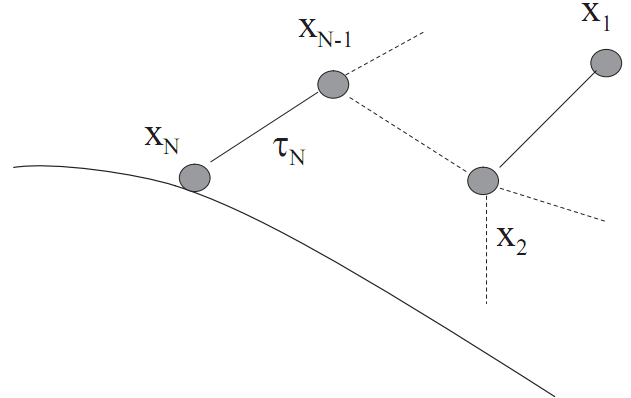
\includegraphics[width=0.55\textwidth]{resonances_decays}
        \caption{The cascade decay in the single freeze-out model. An unstable resonance $x_N$ is formed at the freeze-out hypersurface and travels for the time $\tau_N$ depending on its lifetime and decays. If the products are also resonances ($x_{N-1}$, $x_2$) they decay further until the stable particles are formed ($x_1$)~\cite{therminator}.}
        \label{fig:resonances-decay}
      \end{figure}